% !TEX encoding = UTF-8 Unicode

\documentclass[a4paper]{article}

\usepackage{color}
\usepackage{url}
\usepackage[utf8]{inputenc} % make weird characters work
\usepackage{graphicx}
\usepackage[english,serbian]{babel}
\usepackage[unicode]{hyperref}
\usepackage{amsthm}
\usepackage{amssymb}
\usepackage{amsmath}
\usepackage{chngcntr}
\counterwithin{figure}{section}
\hypersetup{colorlinks,citecolor=green,filecolor=green,linkcolor=blue,urlcolor=blue}
\usepackage{listings}
\usepackage{float}
\usepackage[font=small,labelfont=bf]{caption}
\definecolor{codegreen}{rgb}{0,0.6,0}
\definecolor{codegray}{rgb}{0.5,0.5,0.5}
\definecolor{codeblue}{rgb}{0.0,0,0.82}
\lstdefinestyle{mystyle}{
    numbers=left,
    numberstyle=\scriptsize,
    numbersep=8pt,
    commentstyle=\color{codegray},
    keywordstyle=\color{codegreen},
    numberstyle=\tiny\color{codeblue},
    stringstyle=\color{codegreen},
    basicstyle=\ttfamily\footnotesize,
    breakatwhitespace=false,
    breaklines=true,
    captionpos=b,
    keepspaces=true,
    showspaces=false,
    showstringspaces=false,
    showtabs=false,
    tabsize=4,
    xleftmargin=3em,
    framexleftmargin=1.5em
}
\lstset{style=mystyle}


\theoremstyle{plain}
\newtheorem{thm}{Teorema}[section] % reset theorem numbering for each chapter
\newtheorem{lem}{Lema}[section] % reset theorem numbering for each chapter
\theoremstyle{definition}
\newtheorem{defn}[thm]{Definicija} % definition numbers are dependent on theorem numbers
\newtheorem{exmp}[thm]{Primer} % same for example numbers


\begin{document}

\title{Fibona\v{c}ijev hip\\ \small{Seminarski rad u okviru kursa\\Konstrukcija i analiza algoritama 2\\ Matematički fakultet}}

\author{\href{mailto:ivan_ristovic@math.rs}{Ivan Ristovi\'c}\\\href{mailto:mi14042@matf.bg.ac.rs}{Milana Kovacevi\'c{}}}
\date{januar 2019.}

\maketitle

\abstract{
    Fibona\v{c}ijev hip je struktura podataka osmi\v{s}ljena sa ciljem da pobolj\v{s}a vreme potrebno za operacije nad hipovima. Pru\v{z}aju bolje amortizovano vreme izvr\v{s}avanja nego ve\'c{}ina drugih prioritetnih redova, uklju\v{c}uju\'c{}i binarni i binomni hip. Fibona\v{c}ijev hip je osmi\v{s}ljen 1984. godine i publikovan 1987. Ime je dobio po Fibona\v{c}ijevim brojevima, koji se koriste u analizi slo\v{z}enosti operacija. Koriste\'c{}i Fibona\v{c}ijev hip, mogu\'c{}e je unaprediti vremena izvr\v{s}avanja velikog broja poznatih algoritama kao \v{s}to je Dijsktrin algoritam. Pru\v{z}amo implementaciju Fibona\v{c}ijevog hipa u programskom jeziku \emph{Python}, sa interfejsom jednostavnim za upotrebu i testiranje. Takodje u ovom radu testiramo vreme izvr\v{s}avanja operacije \emph{decrease-key} kako bismo eksperimentalno pokazali konstantno amortizovano vreme izvr\v{s}avanja ove operacije.
}

\tableofcontents

\newpage

\section{Uvod}
\label{sec:Uvod}

\emph{Binarni hip} (eng. \emph{Binary heap}) \cite{Heap} je binarno stablo koje zadovoljava uslov da svaki \v{c}vor u stablu ima vrednost klju\v{c}a ve\'c{}u (tj. manju) od oba svoja sina. Takav hip se \v{c}esto naziva \emph{max-hip} (tj. \emph{min-hip}). Jasno je da \'c{}e se u hipu maksimum (tj. minimum) nalaziti u korenu stabla, \v{s}to garantuje da je operacija pronala\v{z}enja elementa sa maksimalnom (minimalnom) vredno\v{s}\'{c}u konstantne vremenske slo\v{z}enosti. Svaki hip podr\v{z}ava slede\'c{}e operacije \footnote{Pretpostavlja se da se radi o min-hipu, analogno va\v{z}i i za max-hip.}:
\begin{itemize}
    \item \texttt{find\_min} - vra\'c{}a vrednost minimalnog elementa iz hipa.
    \item \texttt{extract\_min} - uklanja minimalni element iz hipa.
    \item \texttt{insert(v)} - unosi novi \v{c}vor sa vredno\v{s}\'c{}u klju\v{c}a $v$.
    \item \texttt{decrease\_key(k,v)} - spu\v{s}ta vrednost klju\v{c}a $k$ na vrednost $v$.
    \item \texttt{merge(h)} - unija sa novim hipom $h$.
\end{itemize}

\emph{Fibona\v{c}ijev hip} \cite{Book} je osmi\v{s}ljen 1984. od strane Fredman-a i Tarjan-a sa ciljem da se pobolj\v{s}a vreme izvr\v{s}avanja Dijkstrinog algoritma za pronala\v{z}enje najkra\'c{}ih puteva. Originalni Dijsktrin algoritam koji koristi binarni hip radi u vremenskoj slo\v{z}enosti $O(|E|\log{|V|})$. Kori\v{s}\'c{}enjem Fibona\v{c}ijevog hipa umesto binarnog hipa, vremensku slo\v{z}enost Dijsktrinog algoritma je mogu\'c{}e pobolj\v{s}ati do $O(|E| + |V|\log{|V|})$. Poredjenje vremena izvr\v{s}avanja u odnosu na binarni hip se mo\v{z}e videti na slede\'c{}oj tabeli:

\begin{table}[H]
\centering
\begin{tabular}{|l|l|l|}
    \hline
    Operacija                   & Binarni hip  & Fibona\v{c}ijev hip \\
    \hline
    \texttt{find\_min}          & $O(1)$       & $O(1)$              \\
    \texttt{extract\_min}       & $O(\log{n})$ & $O(\log{n})$        \\
    \texttt{insert(v)}          & $O(\log{n})$ & $O(1)$              \\
    \texttt{decrease\_key(k,v)} & $O(\log{n})$ & $O(1)$ (amortizovano) \\
    \texttt{merge(h)}           & $O(n)$       & $O(1)$              \\
    \hline
\end{tabular}
\label{tbl:fig1}
\caption{Poredjenje vremena izvr\v{s}avanja operacija izmedju Fibona\v{c}ijevog i binarnog hipa.}
\end{table}

U nastavku \'{c}e biti detaljnije opisana struktura hipa (odeljak \ref{sec:Struktura}) i operacije nad njim (odeljak \ref{sec:Operacije}). U daljem tekstu \'c{}emo pretpostaviti da se radi o min-hipu, analogno va\v{z}i i za max-hip.


\section{Opis strukture}
\label{sec:Struktura}

Fibona\v{c}ijev hip je skup stabala uredjenih po uslovu hipa (videti sliku \ref{fig1}). Koreni tih hipova se \v{c}uvaju u dvostruko povezanoj listi radi lak\v{s}eg ubacivanja i izbacivanja. Takodje se \v{c}uva pokaziva\v{c} na najmanji element, kako bi se upit mogao izvr\v{s}iti u konstantnom vremenu. 

\begin{figure}[H]
    \centering
    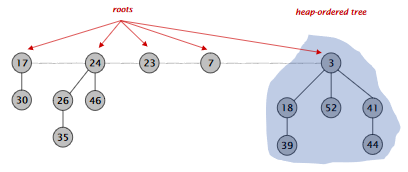
\includegraphics[scale=0.8]{resources/fig1.PNG}
    \caption{Vizuelizacija strukture Fibona\v{c}ijevog hipa.}
    \label{fig1}
\end{figure}

Dodatno, svaki \v{c}vor u sebi sadr\v{z}i podatak da li je ozna\v{c}en ili ne (razlog za\v{s}to \'c{}e biti obja\v{s}njen kasnije). Po\v{s}to hipovi koji \v{c}ine skup ne moraju biti binarni, potreban je neki mehanizam \emph{ispravljanja} hipova \cite{Slides}.

Uvodimo slede\'c{}e pojmove:
\begin{itemize}
    \item $n$ - ukupan broj \v{c}vorova u Fibona\v{c}ijevom hipu.
    \item $rank(x)$ - broj potomaka \v{c}vora $x$.
    \item $rank(H)$ - maksimalni rank bilo kog \v{c}vora u Fibona\v{c}ijevom hipu H.
    \item $trees(H)$ - broj hipova u Fibona\v{c}ijevom hipu H.
    \item $marks(H)$ - broj ozna\v{c}enih \v{c}vorova u Fibona\v{c}ijevom hipu H.
\end{itemize}

Kako bismo analizirali slo\v{z}enosti operacija, potrebno je da prvo defini\v{s}emo \emph{potencijal} Fibona\v{c}ijevog hipa:

\begin{defn}
    \emph{Potencijal} Fibona\v{c}ijevog hipa $H$, u oznaci $\Phi(H)$ se defini\v{s}e kao:
    $$\Phi(H) = trees(H) + 2 \cdot marks(H)$$
\end{defn}


\section{Opis operacija}
\label{sec:Operacije}

\subsection{\texttt{find\_min}}
\label{subsec:findmin}

Pronala\v{z}enje vrednosti minimuma se trivijalno odvija jer imamo pokaziva\v{c} na \v{c}vor koji sadr\v{z}i minimalni element. Slo\v{z}enost ove operacije je, kao i kod obi\v{c}nog binarnog hipa, $O(1)$.

\subsection{\texttt{insert}}
\label{subsec:insert}

Operacija umetanja novog \v{c}vora se odvija u dva dela. Neka je $x$ \v{c}vor koji \v{z}elimo da ubacimo u hip. Prvo se kreira novo stablo sa $x$ kao korenom. To stablo (koje se sastoji samo od \v{c}vora $x$) se ubacuje u listu korena Fibona\v{c}ijevog hipa. Eventualno je potrebno a\v{z}urirati pokaziva\v{c} na najmanji element ukoliko je klju\v{c} \v{c}vora $x$ manji od minimuma hipa. Vizuelni prikaz operacije umetanja se mo\v{z}e videti na slici \ref{fig2}.

Slo\v{z}enost operacije umetanja je stoga $O(1)$, dok je promena u potencijalu $+1$.

\begin{figure}[H]
    \centering
    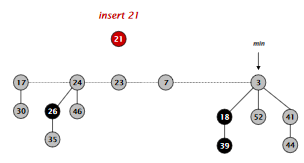
\includegraphics[scale=0.85]{resources/fig2a.PNG}\\
    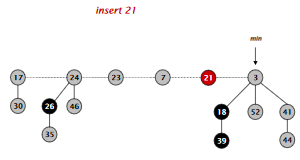
\includegraphics[scale=0.85]{resources/fig2b.PNG}
    \caption{Vizuelizacija operacije umetanja.}
    \label{fig2}
\end{figure}


\subsection{\texttt{extract\_min}}
\label{subsec:extractmin}

Da bismo implementirali operaciju brisanja minumuma, potrebno je prvo da defini\v{s}emo operaciju \emph{spajanja} (eng. \emph{linking}) dva hipa. Naime, porede se koreni dva hipa i kao sin manjeg se dodaje ve\'c{}i (videti sliku \ref{fig3}).

\begin{figure}[H]
    \centering
    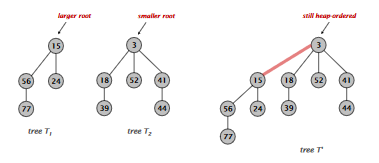
\includegraphics[scale=0.85]{resources/fig3.PNG}
    \caption{Vizuelizacija spajanja hipova.}
    \label{fig3}
\end{figure}

Brisanje se odvija u dva koraka. Prvo se \v{c}vor koji je minimalan izbaci iz liste korenova a njegova deca se ubacuju u listu korenova (videti sliku \ref{fig4a}) i a\v{z}urira se minimum hipa. Zatim se radi \emph{konsolidacija} hipa. Naime, potrebno je pro\'c{}i kroz listu korenova i postarati se da nijedna dva korena nemaju isti rank (videti sliku \ref{fig4b}). Ukoliko dva korena imaju isti rank, njihova stabla se spajaju operacijom spajanja.

Slo\v{z}enost operacije umetanja se analizira tako \v{s}to se analiziraju operacije od kojih se sa\v{c}injena:
\begin{itemize}
    \item Ubacivanje sinova minimalnog \v{c}vora u listu korena je slo\v{z}enosti $O(rank(H))$.
    \item A\v{z}uriranje vrednosti minimuma je slo\v{z}enosti $O(rank(H)) + O(trees(H))$.
    \item Konsolidacija hipa je slo\v{z}enosti $O(rank(H)) + O(trees(H))$.
\end{itemize}
Sve ukupno, $O(rank(H)) + O(trees(H))$.

Promena u potencijalu (ozna\v{c}ena sa $\delta\Phi(H))$) je $O(rank(H) - trees(H))$. Ovo proizilazi iz \v{c}injenice da je $trees(H') = trees(H) + 1$ jer nijedna dva \v{c}vora nemaju isti rank posle konsolidacije. Stoga je $\delta\Phi(H) = rank(H) + 1 - trees(H)$. Iz svega ovoga zaklju\v{c}ujemo da je amortizovana cena operacije brisanja minimuma $O(rank(H))$.

\begin{figure}[H]
    \centering
    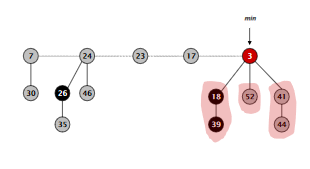
\includegraphics[scale=0.85]{resources/fig4a.PNG}\\
    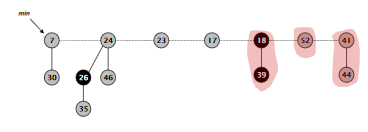
\includegraphics[scale=0.85]{resources/fig4b.PNG}
    \caption{Vizuelizacija prvog koraka operacije brisanja minimuma.}
    \label{fig4a}
\end{figure}
\begin{figure}[H]
    \centering
    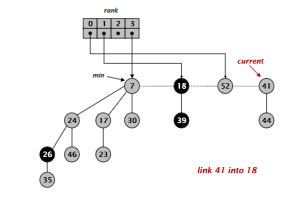
\includegraphics[scale=0.85]{resources/fig4c.PNG}\\
    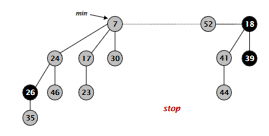
\includegraphics[scale=0.85]{resources/fig4d.PNG}
    \caption{Vizuelizacija drugog koraka operacije brisanja minimuma.}
    \label{fig4b}
\end{figure}


\subsection{\texttt{decrease\_key}}
\label{subsec:decreasekey}

Operacija spu\v{s}tanja klju\v{c}a \v{c}vora $x$ do vrednosti $v$ (eng. \emph{decrease key}) kao rezultat menja vrednost klju\v{c}a \v{c}vora $x$ u $v$ (pretpostavlja se da je $v$  manje od vrednosti klju\v{c}a \v{c}vora $x$). S obzirom da ova operacija mo\v{z}e da naru\v{s}i uslov hipa, potrebno je preurediti hip kako bi se uslov odr\v{zao}.

Operacija spu\v{s}tanja se radi u vi\v{s}e koraka. Intuitivno, ukoliko je uslov hipa ispunjen posle spu{s}tanja vrednosti klju\v{c}a \v{c}vora $x$, onda je posao gotov. U protivnom je potrebno \emph{ise\'c{}i} podstablo \v{c}iji je koren \v{c}vor $x$ i ubaciti ga u skup hipova. Dodatno, ukoliko jednom \v{c}voru ise\v{c}emo i drugog sina, se\v{c}emo i njega i ubacujemo u korenu listu. Ovo radimo rekurizivno dokle god dolazimo do markiranog \v{c}vora ili do korena. Preciznije (videti sliku \ref{fig5}):
\begin{itemize}
    \item Spustiti vrednost klju\v{c}a $x$.
    \item Ise\'c{}i drvo \v{c}iji je $x$ koren, dodati u listu korenova i skloniti oznaku (ukoliko je bio ozna\v{c}en).
    \item Ako je roditelj $p$ \v{c}vora $x$ neozna\v{c}en (nije do sada bio ise\v{c}en), ozna\v{c}iti ga.
    \item U protivnom, ise\'{c}i $p$, dodati ga u listu korenova i skloniti oznaku.
    \item Rekurzivno ponoviti prethoda dva koraka za sve roditelje kojima su dvaput se\v{c}eni sinovi. 
\end{itemize}

Kako bi se osigurala kompleksnost operacije \texttt{extract\_min} i \texttt{decrease\_key}, potrebno je balansirati vrednost funkcije potencijala. Ovo se posti\v{z}e vodjenjem ra\v{c}una o markiranju i brisanju \v{c}vorova, \v{c}ime se odr\v{z}ava \emph{ispravljenost} hipova.
Slo\v{z}enost operacije spu\v{s}tanja klju\v{c}a je $O(c)$, naime potrebno je $O(1)$ vreme za izmenu vrednosti klju\v{c}a i $O(1)$ vreme za svako od $c$ se\v{c}enja, uz dodavanje u listu korenova. Promena potencijala je $O(1) - c$, pa je amortizovana slo\v{z}enost $O(1)$.

Operacija brisanja \v{c}vora $x$ se mo\v{z}e implementirati korist\'c{}i ve\'c{} opisane operacije: prvo \texttt{decrease\_key(}$x$, $-\infty$\texttt{)}  (kako bi se garantovalo da \'c{}e on onda postati minimum hipa) zatim \texttt{extract\_min} (kako bi se taj novonastali minimum uklonio).

\subsection{\texttt{merge}}
\label{subsec:merge}

Unija dva Fibona\v{c}ijeva hipa se trivijalno izvr\v{s}ava spajanjem njihovih dvostruko povezanih listi korenova. Minimum rezultata je manji od dva minimuma hipova koji se spajaju.

\begin{figure}[H]
    \centering
    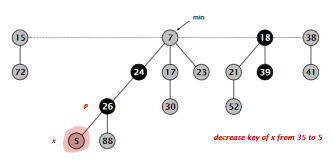
\includegraphics[scale=0.8]{resources/fig5a.PNG}
    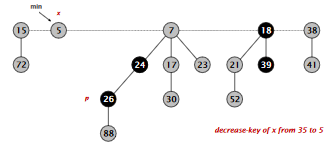
\includegraphics[scale=0.8]{resources/fig5b.PNG}\\
    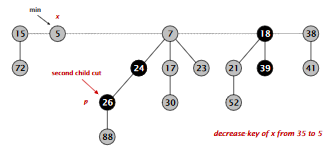
\includegraphics[scale=0.8]{resources/fig5c.PNG}
    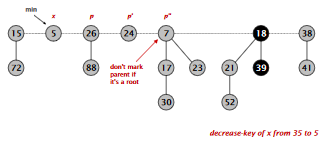
\includegraphics[scale=0.8]{resources/fig5d.PNG}
    \caption{Vizuelizacija operacije spu\v{s}tanja klju\v{c}a.}
    \label{fig5}
\end{figure}

\section{Veza sa Fibona\v{c}ijevim brojevima}
\label{sec:Fib}

\begin{lem}
    Neka je $x$ \v{c}vor i neka su $y_{1}, \dots y_{k}$ njegova deca po redosledu dodavanja u hip. Tada je:
    $$rank(y_{i}) \geq 
    \begin{cases}
        0, & i = 1\\
        i-2, & i \geq 1\\
    \end{cases}
    $$
\end{lem}

A tree of order n has exactly n children.
Trees of order n are formed by taking two trees of order n - 1 and making one the child of another.
If a tree loses two children, that tree is cut away from its parent.

Ozna\v{c}imo sa $F_{k}$ najmanje mogu\'c{}e stablo ranka $k$ koje zadovoljava uslov iznad. Ovakvo stablo je mogu\'{c}e konstruisati ranije opisanim operacijama Fubona\v{c}ijevog hipa. Tokom izvr\v{s}avanja operacije \texttt{extract\_min}, stablo ranka $n$ dobijamo povezivanjem dva stabla ranka $n - 1$. U suprotnom, u operaciji \texttt{decrease\_min}, ukoliko jedan \v{c}vor izgubi dva deteta, i ono samo je odse\v{c}eno od svog roditelja. Ovim osiguravamo da broj \v{c}vorova odgovara Fibona\v{c}ijevim brojevima. Postoji veza - broj \v{c}vorova u $F_{k}$ je ba\v{s} $k$-ti Fibona\v{c}ijev broj:
\begin{figure}[H]
    \centering
    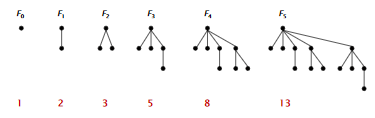
\includegraphics[scale=0.85]{resources/fig6a.PNG}\\
    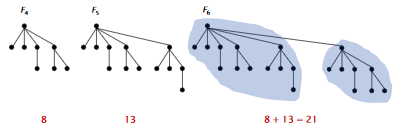
\includegraphics[scale=0.85]{resources/fig6b.PNG}
\end{figure}

S obzirom da je $F_{k} \geq \phi^{k}$, gde je $\phi = (1 + \sqrt{5}) / 2$, dobijamo da je:
$$rank(H) \leq \log_{\phi}{n} $$

Iz ovoga zaklju\v{c}ujemo da je kompleksnost operacije \texttt{extract\_min} $O(\log{n})$.

\section{Poredjenje efikasnosti}
\label{sec:Exp}
Kako bismo ispitali efikasnost na\v{s}e implementacije Fibona\v{c}ijevog hipa, implementirali smo i standardan binarni hip. U narednim podsekcijama su prikazani rezultati poredjenja efikasnosti ova dva hipa.

Poredjenje efikasnosti operacije \texttt{decrease\_key} vr\v{s}imo na slede\'{c}i na\v{c}in:
\begin{itemize}
    \item Kreiramo Fibona\v{c}ijev i binarni hip.
    \item U oba hipa ubacimo $n$ random generisanih vrednosti.
    \item $N$ puta izvr\v{s}imo operaciju na oba hipa i merimo njihovo ukupno vreme izvr\v{s}avanja.
\end{itemize}

\begin{table}[H]
    \centering
    \begin{tabular}{|l|l|l|}
        \hline
        $n$    & Binarni hip           & Fibona\v{c}ijev hip  \\
        \hline
        100    & 0.003965616226196289s & 0.02899909019470215s \\
        1000   & 0.05807352066040039s  & 0.2644772529602051s  \\
        10000  & 0.6527743339538574s   & 3.014829635620117s   \\
        \hline
    \end{tabular}
\label{tbl:fig1}
\caption{\texttt{extract\_min} benchmark}
\end{table}

\begin{table}[H]
    \centering
    \begin{tabular}{|l|l|l|}
        \hline
        $n$    & Binarni hip            & Fibona\v{c}ijev hip    \\
        \hline
        100    & 0.0010502338409423828s & 0.0010502338409423828s \\
        1000   & 0.01744818687438965s   & 0.02191758155822754s   \\
        10000  & 0.2323460578918457s    & 0.293259859085083s     \\
        \hline
    \end{tabular}
\label{tbl:fig1}
\caption{\texttt{decrease\_key} benchmark}
\end{table}


\addcontentsline{toc}{section}{Literatura}
\appendix
\bibliography{references}
\bibliographystyle{plain}

%\appendix
%\section{Dodatak}


\end{document}
